\section{Anhang}
\subsection{Testergebnisse}

\subsection{Abmessungen}

\subsection{Datenblattauszüge}

\textcolor{blue}{Im Anhang befinden sich weitere Detailinformationen des Projekts wie\\
•	Datenblattauszüge, Fertigungsunterlagen (PCB-Layouts, Gehäusezeichnungen, 3D-Druckunterlagen, Montageanleitungen,…) etc.\\
•	sämtliche geforderten Projektmanagementdokumente\\
•	ein Businessplan (optional)
}

\subsection{Projektmanagement}
\textcolor{blue}{In diesem Kapitel soll auf das Projektmanagement des Projektes eingegangen werden. Zu Beginn empfiehlt es sich, die einzelnen Bereiche des Projektmanagements zu erklären und anschließend in einzelnen Kapiteln zu behandeln.}

\subsubsection{Aufgabenstellung des Gesamtprojekts}
\textcolor{blue}{Fügen Sie an dieser Stelle den Text der genehmigten Aufgabenstellung ein, der in die Diplomarbeitsdatenbank  eingegeben wurde.}

\subsubsection{Scrum-Projektplan}
\textcolor{blue}{Fügen Sie hier den vollständigen Scrum-Projektplan, wobei die Nummern der Tasks mit der Arbeitszeitaufzeichnung übereinstimmen müssen. Der Scrum-Projektplan kann auf mehrere Seiten aufgeteilt werden.}

\bgroup
    \centering
    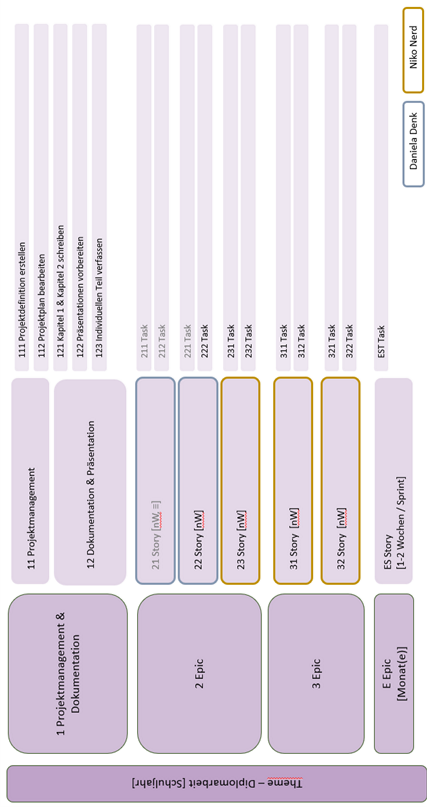
\includegraphics[width=0.6\textwidth]{Scrum_Projektplan_mit_Tasks.png}
    \captionof{figure}{Scrum Projektplan mit Tasks}
\egroup

\newpage
\subsubsection{Terminplanung}

\newpage

\subsubsection{Arbeitspakete}

\paragraph{Maschinenbau (Simbürger)}
\begin{itemize}
    \item Konzeptionierung des Gesamtsystem
    \item CAD - Planung
    \item Komponentenfertigung
    \item Aufbau 
\end{itemize}

\paragraph{Softwareentwicklung (Simbürger)}
\begin{itemize}
    \item Benutzeroberfläche
    \item Warehouse Management System
    \item Datenbanken
\end{itemize}




\newpage

\subsection{Inbetriebnahme}
\color{blue}
Nachdem typische Projekte aus mehreren Komponenten bestehen, ist es oft nicht trivial die einzelnen Komponenten korrekt zu konfigurieren und das Gesamtsystem in Betrieb zu nehmen. In diesem Kapitel soll eine vollständige, präzise und trotzdem möglichst kompak-te Anleitung zur Inbetriebnahme des Systems dargelegt werden. Die Schritte sollen in dem Detailgrad beschrieben werden, dass ein durchschnittlicher Schüler des vierten Jahrganges das Projekt in Betrieb nehmen kann. Exemplarisch sollten Punkte wie die folgenden be-handelt werden – die Aufzählung ist nicht vollständig):
\begin{itemize}
    \item Treiberinstallationen und Systemkonfigurationen
    \item Zu empfehlen wäre bei Server-Installationen ein Setup-Script, welches auf einem vordefinierten Docker-container aufbaut.
    \item Welche Schritte sind notwendig, um das Projekt mit dem vorhandenen Code / Schaltplänen (auf GIT, CD, Netzlaufwerk, etc.) in Betrieb zu nehmen.
    \item Bei Schaltungen mit mehreren Platinen muss beschrieben werden, wie diese mit-einander verbunden werden müssen.
\end{itemize}
\color{black}

\newpage
\subsection{Kostenaufstellung}
\textcolor{blue}{Für die Kalkulation im Gesamtprojekt sind folgende Kosten zu erfassen: \\
•	Kosten für Material (Hard- und Software)\\
•	externe Kosten (z.B.: Zukauf von Sensoren, Funkmodule, spezielle Entwicklungsum-gebungen, etc.) 
}
\begin{figure}[h]
    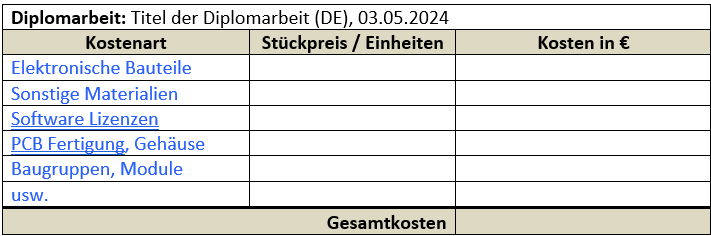
\includegraphics[width=0.8\textwidth]{Kostenaufstellung.png}
    \centering
    \caption{Kostenaufstellung}
\end{figure}

\newpage
\subsection{Besprechungsprotokolle}
%include pdf file as image, on howl page with label
\begin{figure}[H]
    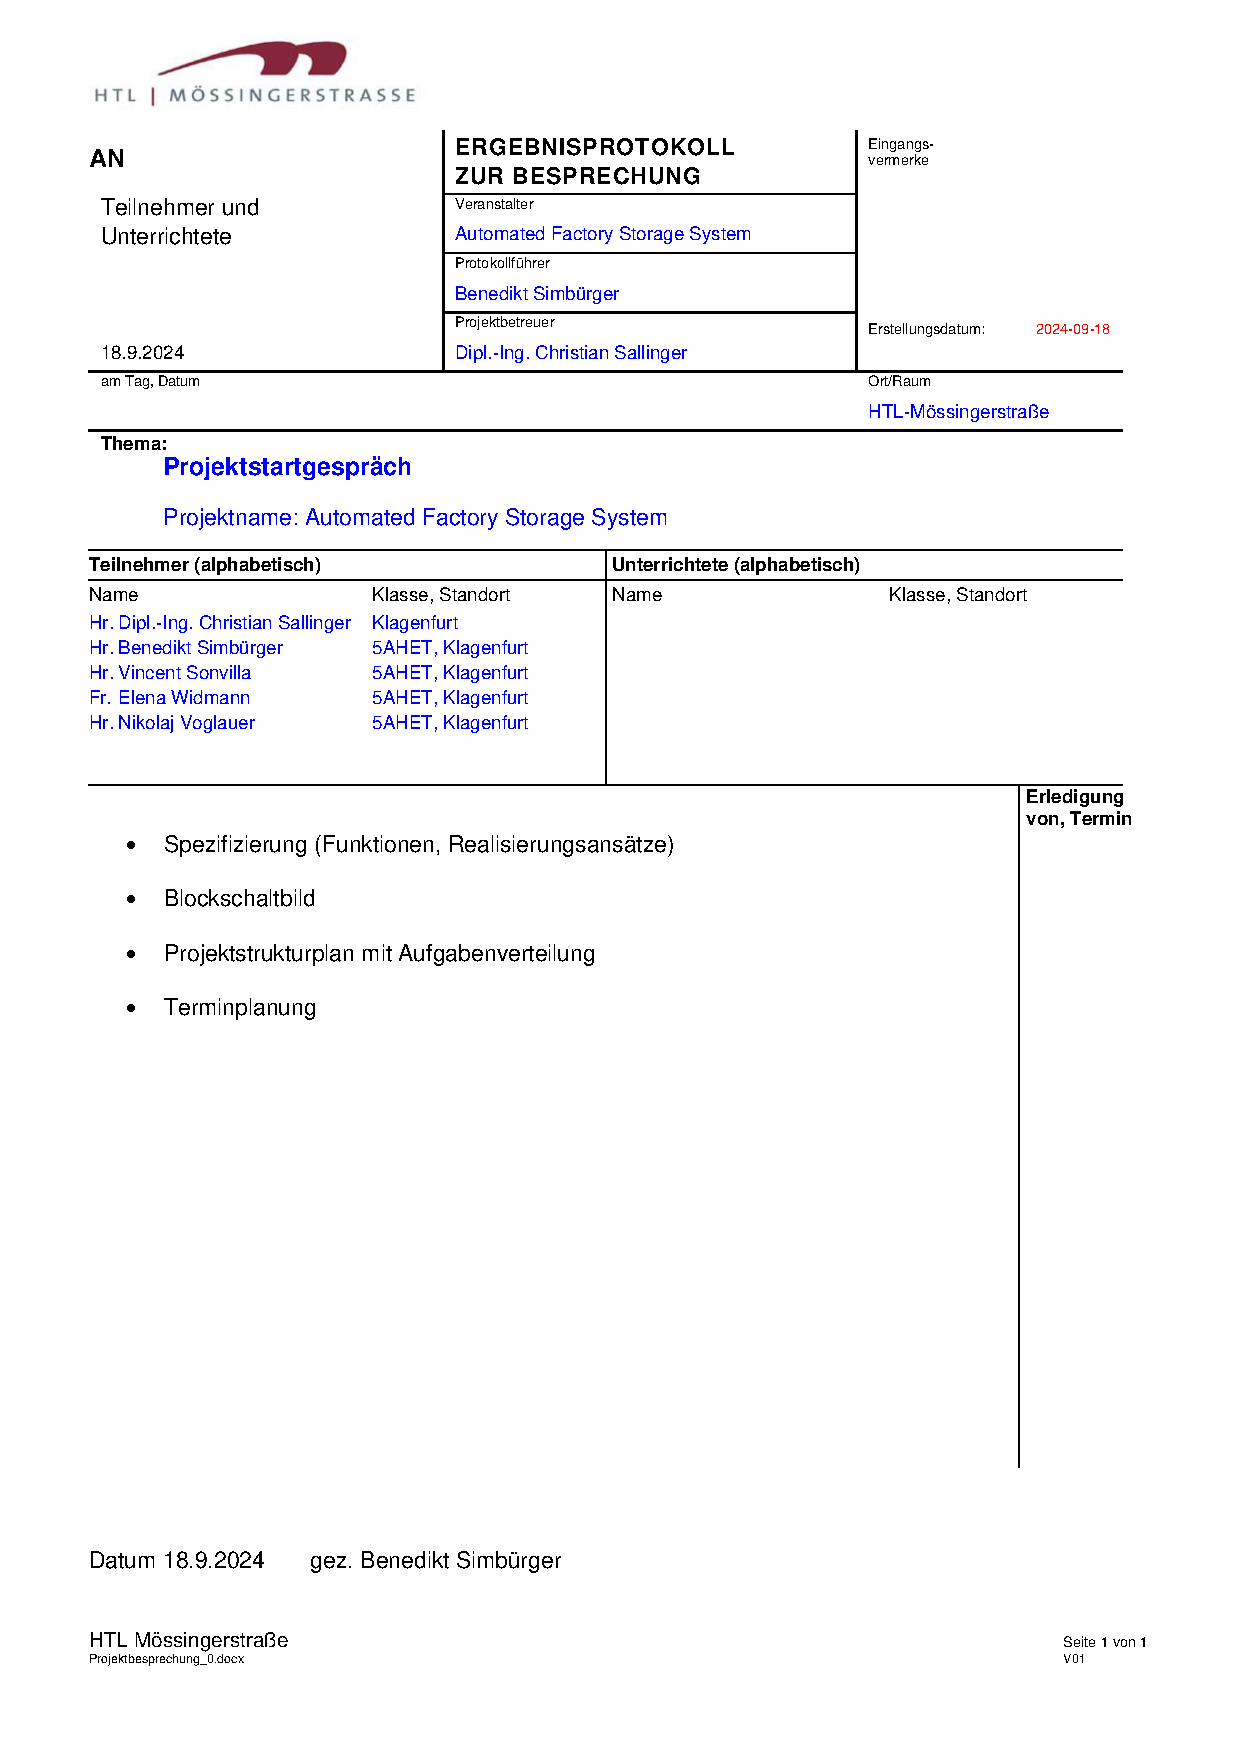
\includegraphics[width=0.9\textwidth]{../Protokolls/Projektbesprechung_0.pdf}
    \centering
    \caption{Besprechungsprotokoll 10.12.2024}
\end{figure}

\begin{figure}[H]
    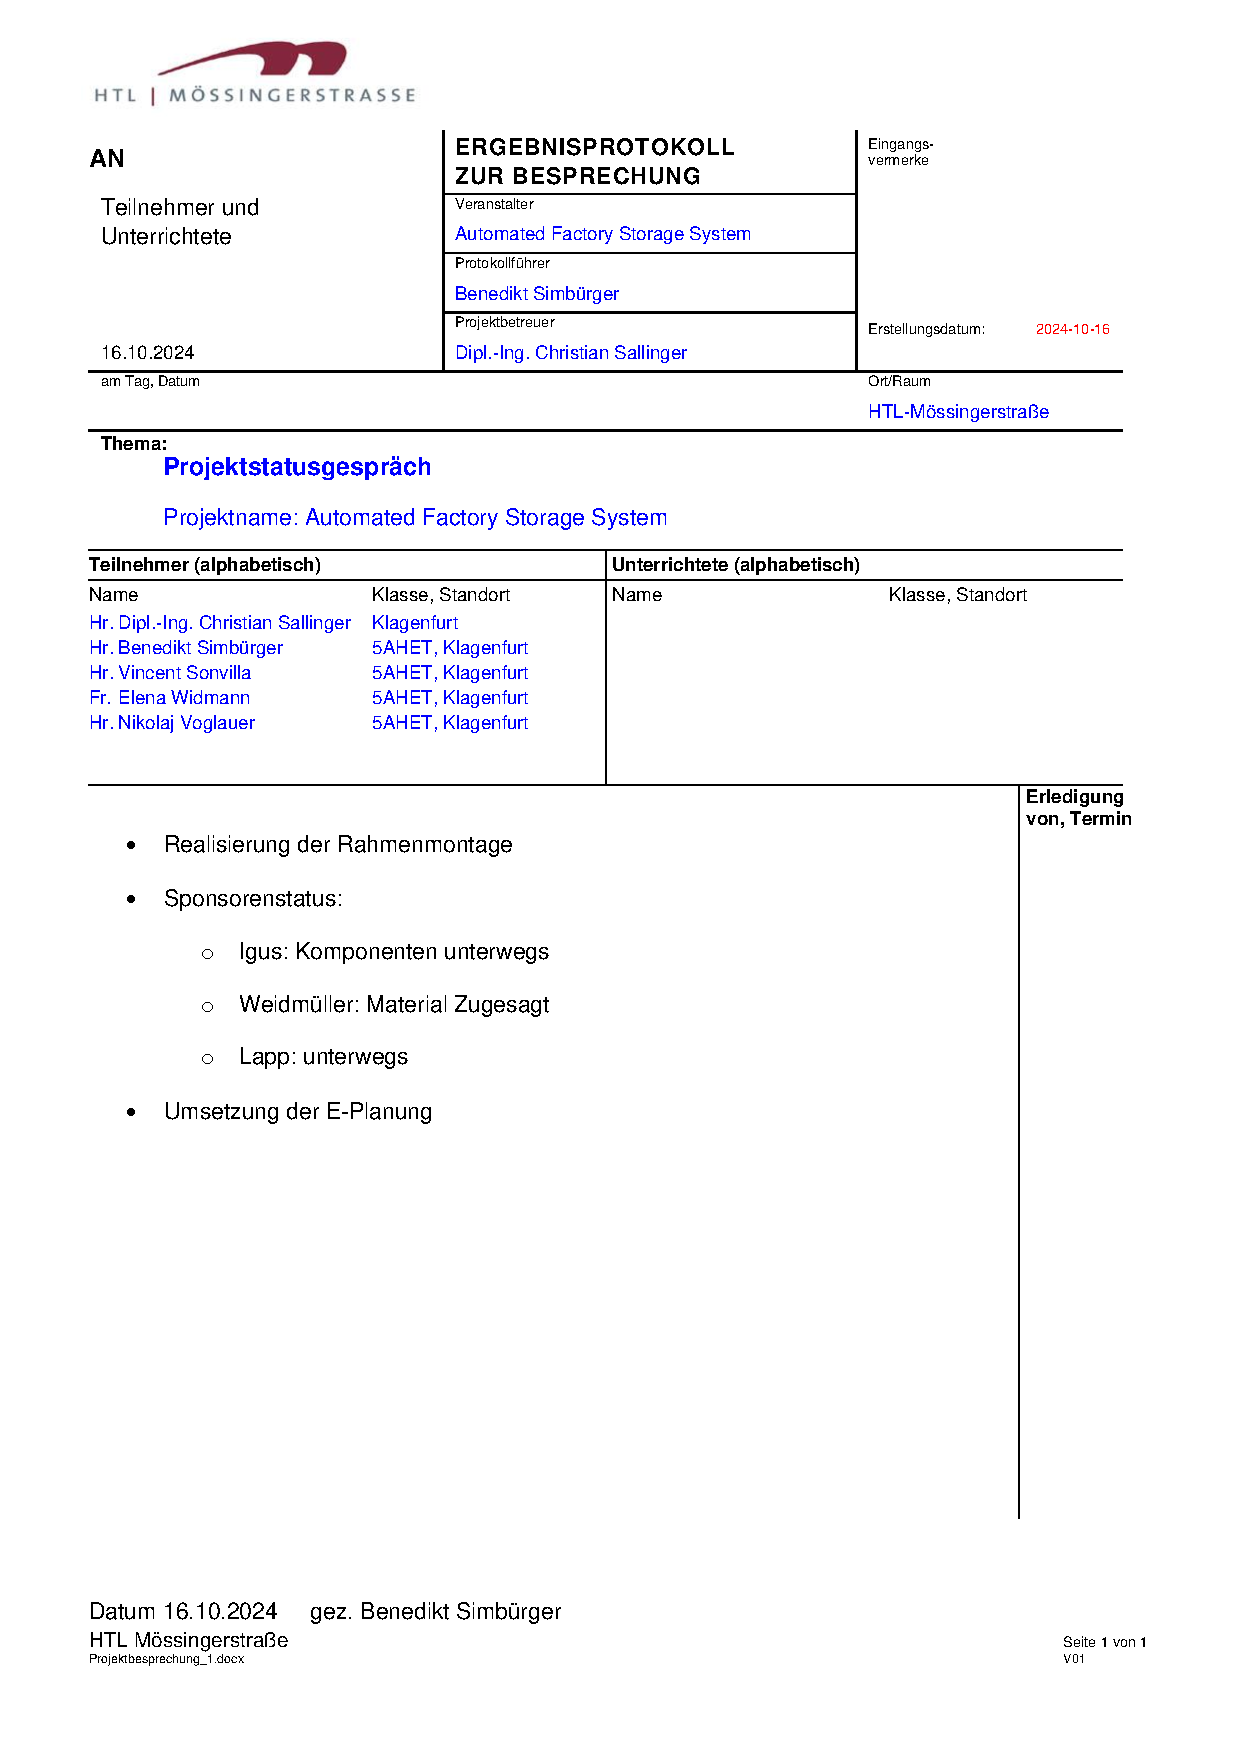
\includegraphics[width=0.9\textwidth]{../Protokolls/Projektbesprechung_1.pdf}
    \centering
    \caption{Besprechungsprotokoll 16.10.2024}
\end{figure}

\begin{figure}[H]
    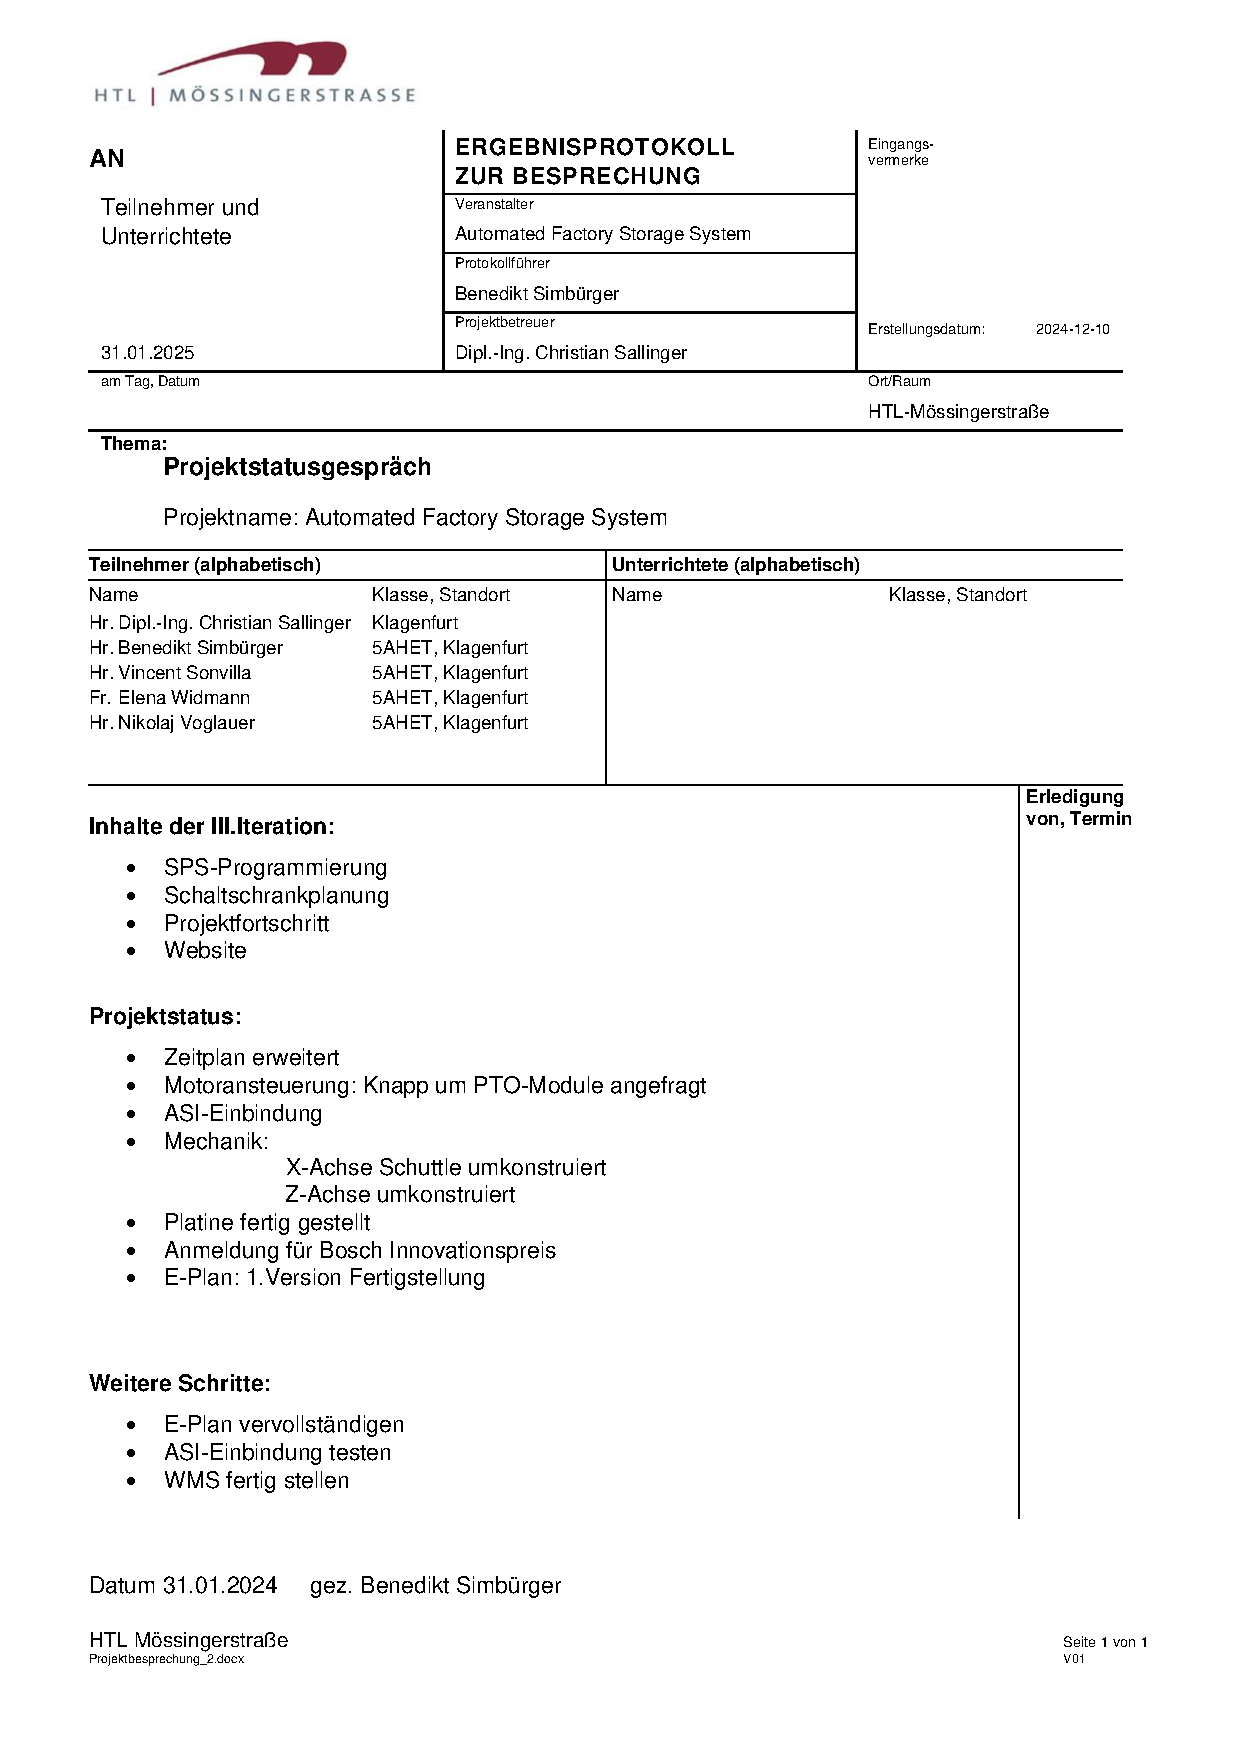
\includegraphics[width=0.9\textwidth]{../Protokolls/Projektbesprechung_2.pdf}
    \centering
    \caption{Besprechungsprotokoll 10.12.2024}
\end{figure}

\begin{figure}[H]
    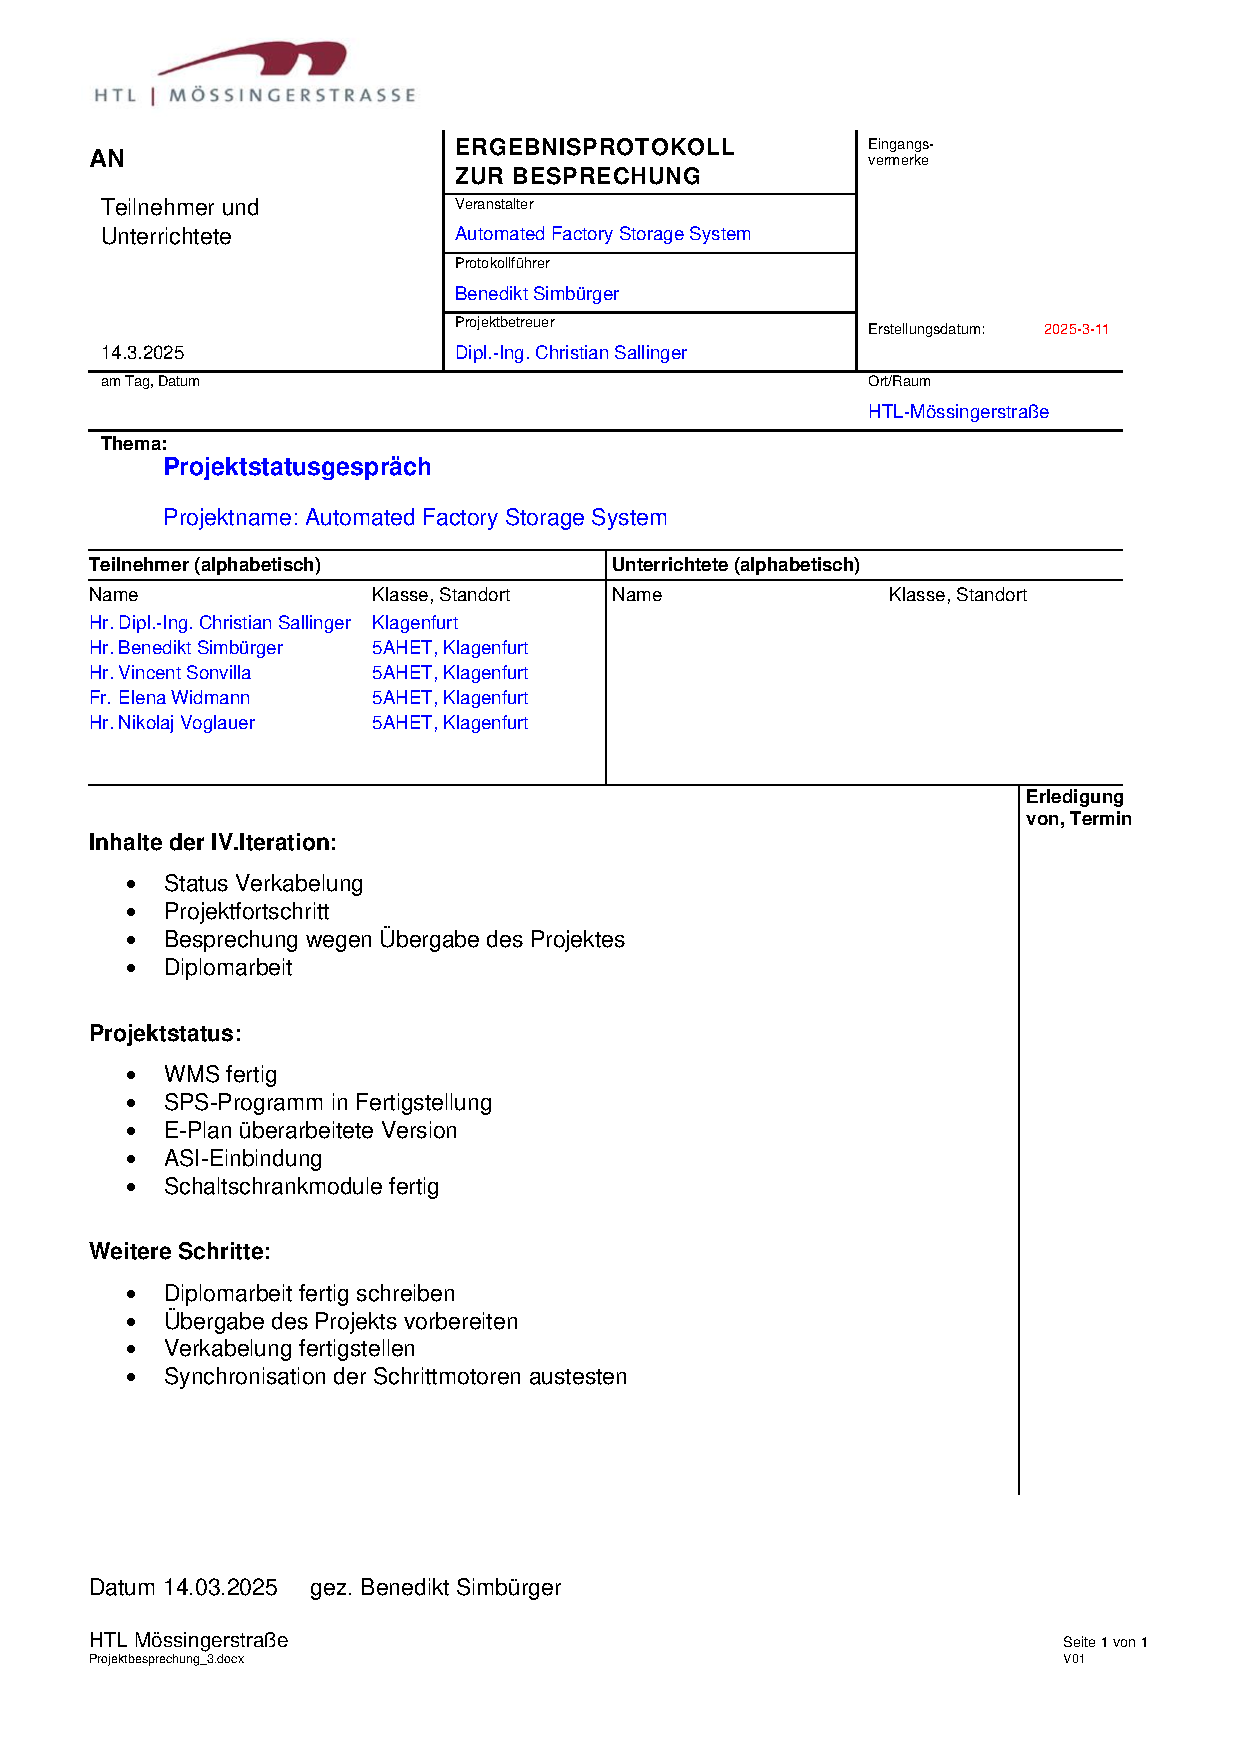
\includegraphics[width=0.9\textwidth]{../Protokolls/Projektbesprechung_3.pdf}
    \centering
    \caption{Besprechungsprotokoll x.x.xxxx}
\end{figure}




\newpage
\subsection{Arbeitsnachweis}

\subsubsection{Simbürger}

\begin{longtable}{|l|p{10cm}|r|}
    \hline
    \textbf{Datum} & \textbf{Tätigkeit} & \textbf{Stunden} \\
    \hline
    \endfirsthead

    \hline
    \textbf{Datum} & \textbf{Tätigkeit} & \textbf{Stunden} \\
    \hline
    \endhead

    \hline
    \endfoot

    \hline
    \endlastfoot

4.10.2023&Besprechung des weiteren vorgehens mit WB	&0.5\\
9.10.2023&Gruppenbesprechung für das weitere Vorgehen	&1.0\\
9.11.2023&Reconstruction Siemens Twin Towers	&3.5\\
14.11.2023&	Reconstruction Siemens Twin Towers	&2.0\\
23.11.2023&	Reconstruction Siemens Twin Towers Lasern	&2.0\\
29.11.2023&	RSTT Ausfahrer + Schlitten Fertigstellung&	4.0\\
19.12.2023	&CAD Auf/Ab-fahrer	&3.0\\
20.12.2023	&CAD RSTT, AutCad vorbereitung	&2.0\\

10.1.2024	&Testversuch ET200 SPS Stepdrive und Meeting Knapp&	4.0\\
11.1.2024	&Achse mechanisch fertig, Schlitten vertikal&	4.0\\
12.1.2024	&CAD Schuttel, Tag der offenen Tür vorbereitung	&2.0\\
16.1.2024	&Motoren ansteuern&	1.0	\\
20.1.2024	&Umlenkungen- und Aufhängungskonstruktion&	4.0\\
29.1.2024	&Diagramm Datenaustausch Anfertigung&   2.0\\
1.2.2024	&Besprechung WB&	4.0\\
3.2.2024	&Website Backend/Frontend Prototyp&	9.0\\
4.2.2024	&WS Frontend&	3.0\\

5.2.2024	&KWF Antrag schreiben und WS Datenbankmanagement&	3.0\\
7.2.2024	&OPC UA Client testung&	4.5\\
15.2.2024	&WS Suche usw, Organisation, Maschinenbaubesprechung	&5.5\\

20.2.2024	&Python / OPC UA Client testen	&1.0\\
23.2.2024	&WS Warenkorb, restructuring	&9.0\\
24.2.2024	&WS Warenkorb fertig, OPC anfang und Pflichtenheft Erstversion&	6.0\\
27.2.2024	&http-Kommunikation	testen&4.0\\
28.2.2024	&Lasten/Pflichtenheft erstellen	&3.0\\
4.3.2024	&http-Kommunikation testen&	3.5\\
10.3.2024	&CAD X-Achse& 7.0\\
13.3.2024	&Absprache mit WB bez. Pflichtenheft	&1.0\\
14.3.2024	&http-Kommunikation und CAD&	3.0\\
1.4.2024	&Datenbanken und Visualisierung	&5.0\\
2.4.2024	&CAD Lagerregal&	2.0\\
17.4.2024	&CAD Gabel und Software&	2.0\\
23.4.2024	&STT-Fortsetzung / Software einführung&	2.5\\
12.4.2024	&Datenbanken und Visu	&5.0\\
21.4.2024	&Datenbanken und Visu	&5.0\\
22.4.2024	&TF-IDF Recherche	&3.0\\
23.4.2024	&TF-IDF Implementierung	&2.0\\
28.4.2024	&Areas und Locations Implementierung	&6.0\\
19.4.2024	&Order Algorithmus konzeptionieren	&3.0\\
22.5.2024	&Order Algorithmus Implementierung	&3.0\\
2.6.2024	&Order Api Programmierung	&5.0\\
3.6.2024	&Api Implementierung und Visu& 3.0\\
4.6.2024	&STT-Fortsetzung und CAD&	2.0\\
6.6.2024	&SPS/Server Communictaion und Z-Prototyp CAD	&5.0\\
8.6.2024	&SPS Comm und Simulation implement	&4.0\\
9.6.2024	&System Controller	&4.0\\

14.6.2024	&Z-Prototyp Bauteile Vorbereitung& 1.0\\
18.6.2024	&Return, Cart programmieren	&4.0\\
19.6.2024	&Docker (f me)	&3.0\\
21.6.2024	&Z-PT, Schaltschrank, SPS-Com&	4.5\\
16.7.2024	&Recherche, Referenz-Elektronik&	1.0\\
17.7.2024	&Ref-Elektronik	&2.0\\
19.7.2024	&Designe/CAD Rollen u. Spannen y &6.0\\
22.7.2024	&Design X-Spannelement	&2.0\\
25.7.2024	&Design X-Spannelement und Rollen	&1.5\\
31.7.2024	&CAD Z-Achsen zauberei &	1.0\\
1.8.2024	&CAD Z-Achse redesign & 5.0\\
9.8.2024	&CAD YZ-Achse grobe fertigstellung&	5.0\\
10.8.2024	&CAD YZ-Achse feinerschliff	&4.0\\
11.8.2024	&CAD YZ-Achse + X-Achse beginn&	2.0\\
12.8.2024	&CAD X-Achse	&1.0\\
13.8.2024	&CAD X-Achse side roller	&4.0\\
14.8.2024	&CAD X-Achse side roller 2. side	&2.0\\
15.8.2024	&CAD X-Achse Mid rollers, side Wheels, YZ-Achse Spiegelung	&6.0\\
16.8.2024	&CAD YZ-Achse Lichttaster, X-Achse	&1.0\\
17.8.2024	&X-Achse Schleppkettengedanken Auslegung	&6.0\\
19.8.2024	&Schleppenderketten einplanung	&2.0\\
20.8.2024	&CAD vertikale Schleppkette &3.0\\
20.8.2024	&Sponsoren-E-mail beginn	&1.3\\
21.8.2024	&Kontaktdaten, Projektzusammenfassung	&1.5\\
22.8.2024	&CAD Schlitten Top 	&1.0\\
24.8.2024	&Stückliste, CAD Schlitten Top	&2.0\\
25.8.2024	&CAD X-Top Verbindung, Umlenkung	&5.0\\
27.8.2024	&CAD Rahmen Aufhängungen	&2.0\\
29.8.2024	&CAD Umlenkungen und Motoraufhängungen	&5.0\\
30.8.2024	&CAD Endschalter und Rahmen beginn	&3.0\\
31.8.2024	&CAD Rahmen, Lagerschrank beginn	&6.0\\
1.9.2024	&CAD Lagerschrank und Querfördererausschnitt	&2.0\\
2.9.2024	&Verbidungsslider implementieren	&1.0\\
3.9.2024	&Bugs beheben, Weidmüller Sortiment Bauteile auswählen	&4.0\\
4.9.2024	&Stack Bug behoben und CAD Querförderer	&7.0\\
5.9.2024	&CAD Mech. weitestgehende Fertigstellung	&4.0\\
9.9.2024	&Latex aufsetzen	&2.5\\
10.9.2024	&Meeting Weidmüller&	2.0	\\
11.9.2024	&Schaltschrank konzeptionieren &2.25\\
15.9.2024	&Stückliste anfertigen	&2.0\\

17.9.2024	&Autolager Demontieren für Bauteilbeschaffung&	2.5\\
18.9.2024	&Verbindungstest, Suchalgorythmus Rust implementation &6.0\\
19.9.2024	&Suchag. Fertig implementiert, CAD Rollen gezeichnet	&3.0\\

24.9.2024	&Projektmanagement&	3.0\\
25.9.2024	&Änderungen V-Slot-Aufhängung, Project-Libre	&1.0\\

26.9.2024	&Igus, Weidmüller, Motoren ansteuern die 1.&	4.0\\
28.9.2024	&Bux im Lageralgorithmus beheben	&1.5\\

1.10.2024	&CAD	&1.0\\
3.10.2024	&Profile bearbeiten	&1.5\\
8.10.2024	&Latex Vorlage	&1.0\\
9.10.2024	&Raumeinrichtung&	3.0\\
21.10.2024	&Rahmenbau beginn&	2.0\\
22.10.2024	&Rahmenbau und Drehstromverlegung, Auftragsvorbereitung X-Aufhängung &5.5\\
23.10.2024	&Rahmenbau	&3.0\\
24.10.2024	&Rahmenbau	&3.0\\
25.10.2024	&CAD XZ-Redesign	&3.0	\\
26.10.2024	&CAD XZ-Redesign	&7.0	\\
27.10.2024	&Auftragsvorbereitung X-Achse	&3.0\\
28.10.2024	&Auftragsvorbereitung X-Achse	&2.0	\\

5.11.2024	&Beginn Umlenkrollen Drehen	&0.8\\
6.11.2024	&Weidmüller DP Inbetrtiebnahme&	1.0\\
7.11.2024	&Weidmülller DP ansteuern&	3.5\\
8.11.2024	&Weidmülller DP ansteuern&	3.5\\
12.11.2024	&Umlenkrollen Drehen &	3.5\\
19.11.2024	&Umlenkrollen Drehen, Fräsen	&2.5\\
20.11.2024	&DAS: Drehen	&1.0\\
21.11.2024	&DAS: TFIDF	&2.0\\
22.11.2024	&DAS	&4.5\\
23.11.2024	&API stack , DAS	&3.0\\
24.11.2024	&DAS	&2.0\\
25.11.2024	&DAS	&1.5\\

26.11.2024	&Drehen& 3.5\\
29.11.2024	&DAS& 4.0\\
3.12.2024	&Drehen, DAS: Maschinenbau& 5.0\\
6.12.2024	&Website, DAS &3.5\\
10.12.2024	&DAS: Software, CAD	&5.0\\
13.12.2024	&Drehen &3.5\\
7.1.2025	&CNC-Fräsen, Hülsen Drehen&	3.5\\
8.1.2025	&X-Achse Zusammenbauen anfangen	&2.0\\
10.1.2025	&X-Achse Zusammenbauen	&4.0\\
14.1.2025	&X-Achse Zusammenbauen &	4.0\\
15.1.2025	&X-Achse Zusammenbauen &	4.5\\
17.1.2025	&Tag der offenen Türe	&5.0\\
21.1.2025	&TIA Portal Verbindung&	3.5\\
24.1.2025	&Lasern, Förderband, Mechanik	&3.5\\
4.2.2025	&Sicherheitstechnik-Besprechung, SPS - Server Kommunikation	&3.5\\
14.2.2025	&WMS Location Updateing	&1.0\\
17.2.2025	&DAS: Allgemeinteil	&1.0\\
21.2.2025	&Ref, Fräsen, Da-Schreiben	&5.0\\
25.2.2025	&Zusammenbauen&	4.0\\
28.2.2025	&Fräsen, E-Plan,&	3.5\\
2.3.2025	&DAS: Aufbau	&1.5\\
3.3.2025	&DAS: Besprechungsprotokolle&	1.0\\
5.3.2025	&Umlenkung und Motoren einbauen&	4.5\\
6.5.2025	&DAS  &	2.5\\
9.3.2025	&DAS XZ-Achse	&1.0\\
10.3.2025	&DAS	&3.0\\
11.3.2025	&DAS	&3.0\\
14.3.2025	&Verkabelung Schaltschrank	&4.0\\


    
\end{longtable}


\newpage
